\begin{frame}{Physical Setup}
\begin{block}{Physical System Under Consideration}
\begin{itemize}
	\item Countable state-space $\mathcal{X}$
	\item Connected to a work reservoir
	\item Connected to heat bath at temperature $T$
	\begin{itemize}
		\item Bath in a Boltzmann distribution
	\end{itemize}
	\item System evolves according to driving protocol during time interval $[0,t_f]$
\end{itemize}
The heat function $Q(x)$ is the expected thermal energy transferred from the system to the heat bath.
\end{block}
\end{frame}
\begin{frame}{Physical Setup}

    \begin{figure}
            \centering
            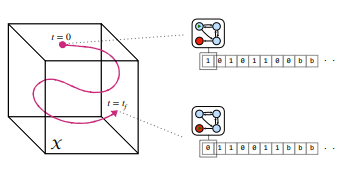
\includegraphics{System.png}
            \label{fig:system_visual}
        \end{figure}
\end{frame}

\begin{frame}{Physical Setup}
\begin{block}{System under consideration}
The joint Hamiltonian of the system is
\begin{equation*}
    H_X^t(x) + H_B(b) + H_{\text{int}}(x,b)
\end{equation*}
If $p_B(b)$ is the initial distribution of the bath and $p'_{B|X}$ is the final distribution, then:
\begin{equation*}
    Q(x) = \langle H_B \rangle_{p'_{B|x}} - \langle H_B \rangle_{p_B}
\end{equation*}
\end{block}
\end{frame}




